% Version antislop de body.tex (texto reescrito y codigo de ../antislop/mcnvt.f90).
% Mismos resultados, figuras y tablas que body.tex.

% ============================================================================
% PART 1 (Steps 1-3): el codigo MC, sin serie en densidad
% RESPONSABLE: Torret (toda la seccion)
% ============================================================================
\section{Part 1 (Steps 1--3)}

\subsection{Question}
Determine the equation of state of a Lennard-Jones fluid for the isotherm $T^*=2.0$ with a personal Monte Carlo code ($N\sim 500$ atoms):
\begin{enumerate}
  \item Write a MC code for an $(N,V,T)$ simulation of a Lennard-Jones system, using \texttt{leapfroglj.f} as the starting point.
  \item Compute the interaction energy $U=\langle\sum_i\sum_{j>i}U(r_{ij})\rangle$ and the pressure $P=\rho k_BT+\frac{1}{3V}\langle\sum_i\sum_{j>i}\vec r_{ij}\cdot\vec F_{ij}\rangle$, with their standard deviations $\sigma_U$ and $\sigma_P$.
  \item Compute the radial distribution function $g(r)$.
\end{enumerate}

\subsection{Code}
We turned \texttt{leapfroglj.f90} from Practice~2 into the Monte Carlo program \texttt{mcnvt.f90}, following the changes the teacher marked on \texttt{leapfroglj.f}: the velocities and accelerations go away, \texttt{velpos} becomes the trial move \texttt{mcmove}, and \texttt{lj} only has to return the pair energy. The program uses reduced units ($\sigma=\epsilon=k_B=1$), $N=500$ atoms in a cubic box with periodic boundary conditions and the minimum image convention, and the Lennard-Jones potential cut at $r_c=2.5\sigma$. The full source is in the Annex.

In each trial move (Step~1) we pick one atom at random, shift it by a random amount between $-\Delta/2$ and $\Delta/2$ along each axis, and accept the new position with probability $\min\{1,e^{-\beta\,\delta U}\}$. The energy change $\delta U$ only involves the moved atom, so \texttt{ener} sums its $N-1$ pair energies before and after the move.
\lstinputlisting[style=fortranstyle,firstline=262,lastline=296,firstnumber=262,caption={Metropolis move \texttt{mcmove}.},label={lst:mcmove}]{../antislop/mcnvt.f90}

Every \texttt{nsamp} moves, \texttt{sample} goes over all pairs once and returns $U$ and the virial pressure, while \texttt{lj} adds each pair to the $g(r)$ histogram (Steps~2--3). This is the \texttt{forces} loop of Practice~2 without the accelerations. Both $U$ and $P$ include the tail corrections of a uniform fluid beyond $r_c$,
\begin{equation}
  \frac{U_{\mathrm{tail}}}{N}=\frac{8\pi}{3}\rho\Big(\frac{1}{3r_c^9}-\frac{1}{r_c^3}\Big),\qquad
  P_{\mathrm{tail}}=\frac{16\pi}{3}\rho^2\Big(\frac{2}{3r_c^9}-\frac{1}{r_c^3}\Big).
\end{equation}
\lstinputlisting[style=fortranstyle,firstline=49,lastline=52,firstnumber=49,caption={Tail corrections (same lines as in Practice~2).},label={lst:tail}]{../antislop/mcnvt.f90}
\lstinputlisting[style=fortranstyle,firstline=144,lastline=167,firstnumber=144,caption={Subroutine \texttt{sample}: $U$ and $P$ of the current configuration.},label={lst:sample}]{../antislop/mcnvt.f90}

$\sigma_U$ and $\sigma_P$ are the standard deviations of the 2000 values sampled in each run.

\subsection{Results}
Figure~\ref{fig:traces} shows one run of the program: the $\rho^*=0.5$ point of the Part~2 series, $10^7$ moves from an fcc lattice. The run gives $U^*/N=-3.152$ with $\sigma_U=0.051$ and $P^*=1.067$ with $\sigma_P=0.154$, with $46\%$ of the moves accepted at $\Delta^*=0.527$. Its $g(r)$ is the $\rho^*=0.5$ curve of Figure~\ref{fig:gdr}.

\begin{figure}[H]
  \centering
  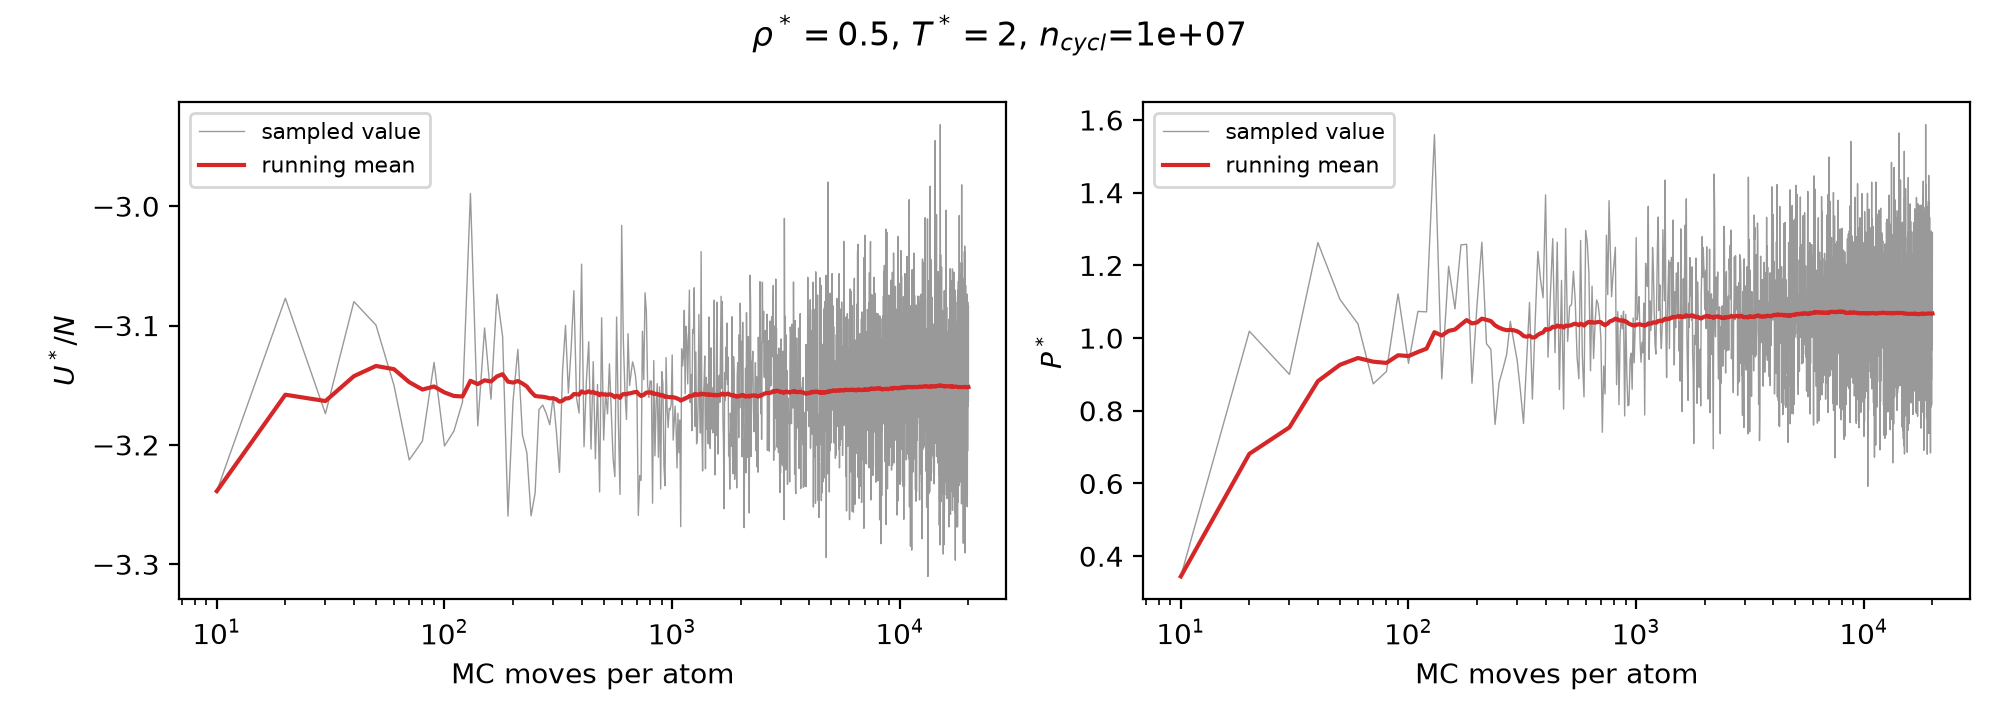
\includegraphics[width=\linewidth]{../figures/traces_rho05.png}
  \caption{Sampled $U^*/N$ (left) and $P^*$ (right) along one MC run at $\rho^*=0.5$, $T^*=2.0$ (one sample every $10$ moves per atom), with their running means. Logarithmic horizontal axis.}
  \label{fig:traces}
\end{figure}

\subsection{Discussion \& Notes}
A trial move costs $O(N)$, since only the $N-1$ pairs of the moved atom change, while a full pass over all pairs costs $O(N^2)$. That is why the program computes $U$, the virial and $g(r)$ only every \texttt{nsamp} moves.

The fcc lattice melts almost at once at $T^*=2$: the first sample, after $10$ moves per atom, is already at $U^*/N=-3.24$, against a mean of $-3.15$. The running mean of $U$ stops changing after about $10^2$ moves per atom and that of $P$ after about $10^3$, out of $2\times10^4$, so we kept all the samples in the averages.

With $r_c=2.5\sigma$ the tail correction to the pressure is $-0.27$ at $\rho^*=0.5$, a quarter of $P^*$, so it cannot be left out. It assumes $g(r)=1$ beyond $r_c$; Part~2 checks this.

$\sigma_U$ and $\sigma_P$ measure how much the instantaneous values fluctuate (the width of the grey band in Figure~\ref{fig:traces}). They are not the error of the mean, which is much smaller after averaging $2000$ samples. The relative fluctuation of $P$ is $14\%$ against $1.6\%$ for $U$, because the virial depends mostly on the steep repulsive part of the potential, where a small change in the distance of a close pair changes the force a lot.

% ============================================================================
% PART 2 (Steps 4-7): serie en densidad rho* = 0.1-0.8
% RESPONSABLE: Montull, salvo los parrafos de Discussion marcados Torret
% ============================================================================
\newpage
\section{Part 2 (Steps 4--7)}

\subsection{Question}
\begin{enumerate}
  \setcounter{enumi}{3}
  \item Perform a series of MC simulations at $T^*=2.0$ and densities from $\rho^*=0.1$ to $0.8$, with $n_{\mathrm{cycl}}\sim10^6,10^7$. List the technical parameters (number of cycles, displacement $\Delta$, acceptance rate, cutoff $r_c$) and the results ($U,\sigma_U,P,\sigma_P$).
  \item Plot $U^*$ and $P^*$ as a function of $\rho^*$. Up to what density is the ideal gas law $P=\rho k_BT$ a good approximation?
  \item Plot $g(r)$ for the different densities.
  \item Obtain $U$ and $P$ by numerical integration of $g(r)$,
  \begin{equation}
    U=2\pi\rho N\!\int_0^\infty\! U(r)g(r)r^2dr,\qquad P=\rho k_BT-\frac{2\pi}{3}\rho^2\!\int_0^\infty\!\frac{dU(r)}{dr}g(r)r^3dr,
  \end{equation}
  and compare with the direct results of Step~4.
\end{enumerate}

\subsection{Code}
The Fortran program is the one of Part~1, unchanged. \texttt{run\_series.py} runs the series of Step~4: for each $\rho^*$ it writes an fcc lattice of $500$ atoms, adjusts $\Delta$ with short runs until about half of the moves are accepted, and then launches the production run. For $\rho^*\le0.3$ the acceptance stays above $50\%$ even at the largest step we allowed, $\Delta^*=0.881$. \texttt{integrar\_gdr.py} does Step~7: it integrates the saved $g(r)$ (500 bins up to $L/2$) from $0$ to $r_c$ with the rectangle rule and adds the same tail corrections. \texttt{plot\_eos.py} makes the figures.

\subsection{Results}
Tables~\ref{tab:n1000000} and~\ref{tab:n10000000} give the technical parameters and the results of the two series, $n_{\mathrm{cycl}}=10^6$ and $10^7$ moves ($2000$ and $20000$ moves per atom), both with $r_c^*=2.5$.

\begin{table}[H]\centering\small
\caption{Technical parameters and results for $n_{\mathrm{cycl}}=10^6$ ($N=500$, $T^*=2.0$, $r_c^*=2.5$). $\sigma_U$ and $\sigma_P$ are the standard deviations of the sampled values (2000 samples per run, one every $n_{\mathrm{cycl}}/2000$ moves). $U$ is per atom and includes the tail correction.}
\label{tab:n1000000}
\begin{tabular}{ccccccc}\hline
$\rho^*$ & $\Delta^*$ & acc.\ (\%) & $U^*/N$ & $\sigma_U$ & $P^*$ & $\sigma_P$ \\ \hline
0.1 & 0.881 & 77.3 & -0.6571 & 0.035 & 0.1774 & 0.013 \\
0.2 & 0.881 & 61.8 & -1.3091 & 0.043 & 0.3306 & 0.037 \\
0.3 & 0.881 & 49.4 & -1.9217 & 0.046 & 0.4854 & 0.068 \\
0.4 & 0.666 & 47.7 & -2.5357 & 0.047 & 0.6958 & 0.118 \\
0.5 & 0.527 & 46.0 & -3.1540 & 0.049 & 1.0642 & 0.172 \\
0.6 & 0.393 & 48.1 & -3.7522 & 0.065 & 1.7310 & 0.269 \\
0.7 & 0.342 & 44.7 & -4.3099 & 0.085 & 2.9960 & 0.388 \\
0.8 & 0.290 & 43.1 & -4.7791 & 0.128 & 5.1621 & 0.615 \\
\hline\end{tabular}\end{table}
\begin{table}[H]\centering\small
\caption{Technical parameters and results for $n_{\mathrm{cycl}}=10^7$ ($N=500$, $T^*=2.0$, $r_c^*=2.5$). $\sigma_U$ and $\sigma_P$ are the standard deviations of the sampled values (2000 samples per run, one every $n_{\mathrm{cycl}}/2000$ moves). $U$ is per atom and includes the tail correction.}
\label{tab:n10000000}
\begin{tabular}{ccccccc}\hline
$\rho^*$ & $\Delta^*$ & acc.\ (\%) & $U^*/N$ & $\sigma_U$ & $P^*$ & $\sigma_P$ \\ \hline
0.1 & 0.881 & 77.1 & -0.6644 & 0.029 & 0.1777 & 0.013 \\
0.2 & 0.881 & 61.7 & -1.3064 & 0.037 & 0.3294 & 0.038 \\
0.3 & 0.881 & 49.4 & -1.9245 & 0.043 & 0.4893 & 0.070 \\
0.4 & 0.666 & 47.5 & -2.5384 & 0.046 & 0.7045 & 0.110 \\
0.5 & 0.527 & 46.1 & -3.1516 & 0.051 & 1.0673 & 0.154 \\
0.6 & 0.393 & 47.9 & -3.7529 & 0.056 & 1.7403 & 0.204 \\
0.7 & 0.342 & 44.6 & -4.3057 & 0.067 & 3.0182 & 0.279 \\
0.8 & 0.290 & 42.8 & -4.7612 & 0.079 & 5.2534 & 0.353 \\
\hline\end{tabular}\end{table}
\begin{table}[H]\centering\small
\caption{Direct averages (Step~4, $n_{\mathrm{cycl}}=10^7$) against numerical integration of $g(r)$ (Step~7), both with tail corrections.}
\label{tab:integral}\begin{tabular}{ccccccc}\hline
$\rho^*$ & $U_{\mathrm{dir}}$ & $U_{\mathrm{int}}$ & $\Delta U$ & $P_{\mathrm{dir}}$ & $P_{\mathrm{int}}$ & $\Delta P$ \\ \hline
0.1 & -0.6644 & -0.6639 & +0.0006 & 0.1777 & 0.1780 & +0.0003 \\
0.2 & -1.3064 & -1.3058 & +0.0006 & 0.3294 & 0.3301 & +0.0007 \\
0.3 & -1.9245 & -1.9235 & +0.0010 & 0.4893 & 0.4910 & +0.0017 \\
0.4 & -2.5384 & -2.5375 & +0.0010 & 0.7045 & 0.7066 & +0.0021 \\
0.5 & -3.1516 & -3.1504 & +0.0012 & 1.0673 & 1.0706 & +0.0033 \\
0.6 & -3.7529 & -3.7516 & +0.0013 & 1.7403 & 1.7443 & +0.0040 \\
0.7 & -4.3057 & -4.3041 & +0.0017 & 3.0182 & 3.0243 & +0.0061 \\
0.8 & -4.7612 & -4.7592 & +0.0020 & 5.2534 & 5.2614 & +0.0080 \\
\hline\end{tabular}\end{table}
\begin{table}[H]\centering\small
\caption{Comparison with Johnson, Zollweg and Gubbins (1993) at $T^*=2.0$ ($10^7$ cycles; their $r_c$ is $5\sigma$ to $4.27\sigma$, ours $2.5\sigma$ plus tail). The number in parentheses is the error in the last digit(s).}
\label{tab:johnson}\begin{tabular}{cccccc}\hline
$\rho^*$ & $P^*$ (this work) & $P^*$ (Johnson) & $U^*/N$ (this work) & $U^*/N$ (Johnson) & $\Delta P/P$ (\%) \\ \hline
0.1 & 0.1777 & 0.1777(2) & -0.6644 & -0.667(1) & -0.0 \\
0.2 & 0.3294 & 0.3290(6) & -1.3064 & -1.306(1) & +0.1 \\
0.3 & 0.4893 & --- & -1.9245 & --- & --- \\
0.4 & 0.7045 & 0.705(1) & -2.5384 & -2.538(2) & -0.1 \\
0.5 & 1.0673 & 1.069(3) & -3.1516 & -3.149(2) & -0.2 \\
0.6 & 1.7403 & 1.756(7) & -3.7529 & -3.746(2) & -0.9 \\
0.7 & 3.0182 & 3.024(7) & -4.3057 & -4.300(2) & -0.2 \\
0.8 & 5.2534 & 5.28(1) & -4.7612 & -4.753(3) & -0.5 \\
\hline\end{tabular}\end{table}
\begin{table}[H]\centering\small
\caption{Ideal-gas test at $T^*=2.0$ ($10^7$ cycles): compressibility factor $Z=P^*/(\rho^*T^*)$; $Z=1$ for an ideal gas.}
\label{tab:ideal}\begin{tabular}{cccc}\hline $\rho^*$ & $\rho^*T^*$ & $P^*$ & $Z$ \\ \hline
0.1 & 0.20 & 0.1777 & 0.888 \\
0.2 & 0.40 & 0.3294 & 0.823 \\
0.3 & 0.60 & 0.4893 & 0.816 \\
0.4 & 0.80 & 0.7045 & 0.881 \\
0.5 & 1.00 & 1.0673 & 1.067 \\
0.6 & 1.20 & 1.7403 & 1.450 \\
0.7 & 1.40 & 3.0182 & 2.156 \\
0.8 & 1.60 & 5.2534 & 3.283 \\
\hline\end{tabular}\end{table}

\begin{figure}[H]
  \centering
  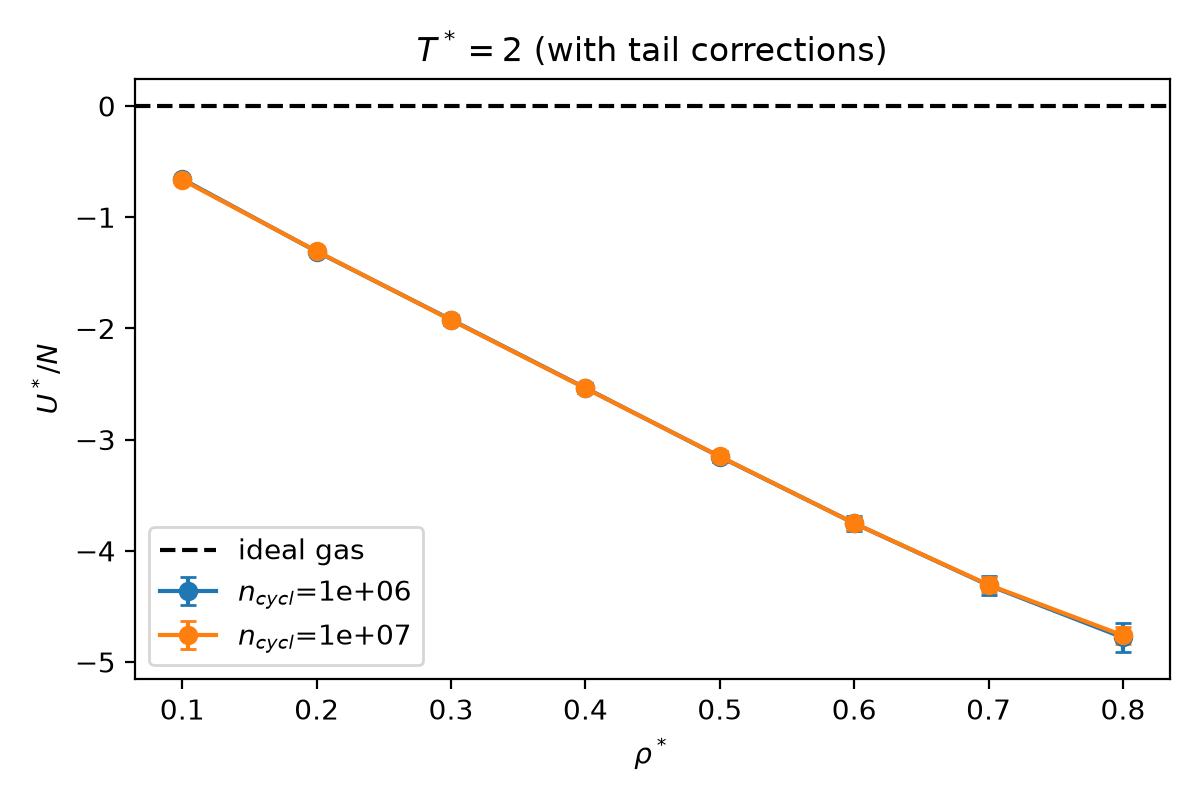
\includegraphics[width=0.48\linewidth]{../figures/U_vs_rho.png}\hfill
  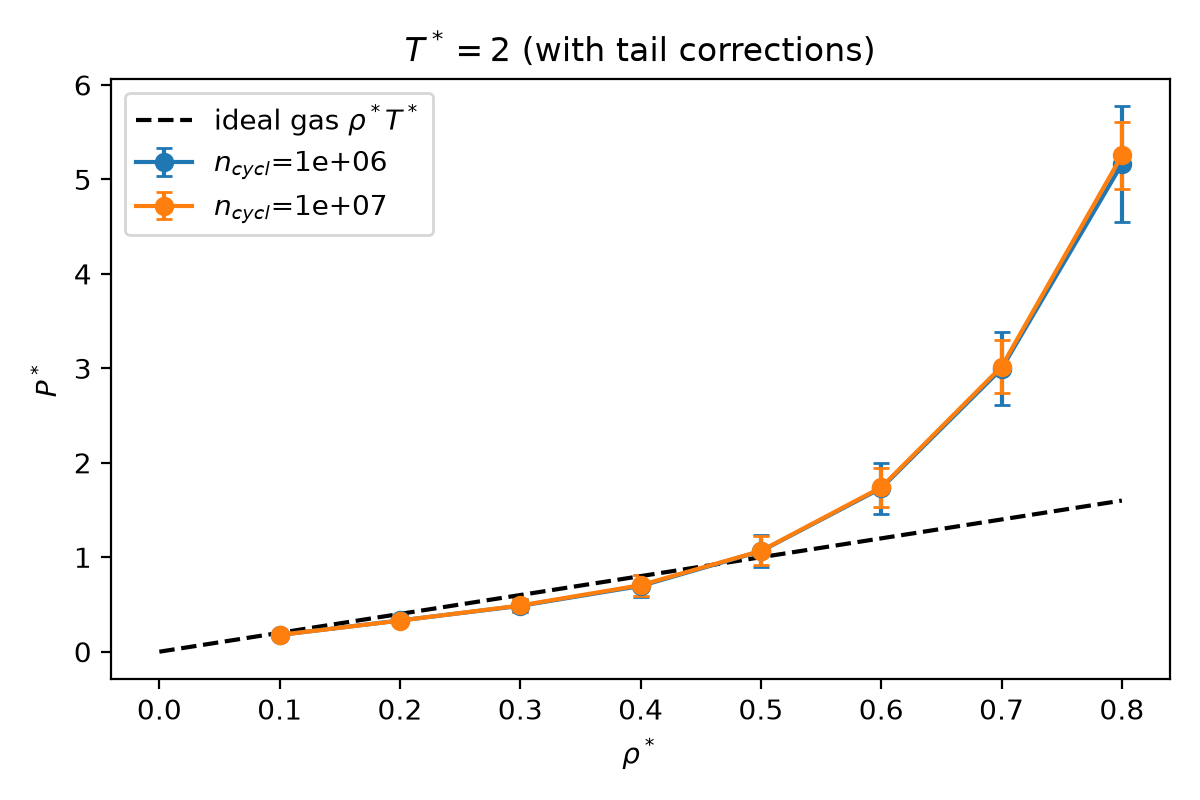
\includegraphics[width=0.48\linewidth]{../figures/P_vs_rho.png}
  \caption{$U^*/N$ (left) and $P^*$ (right) as a function of $\rho^*$ at $T^*=2.0$ for both series; error bars are $\sigma_U$ and $\sigma_P$. The dashed line of the right panel is the ideal gas $P^*=\rho^*T^*$.}
  \label{fig:eos}
\end{figure}

\begin{figure}[H]
  \centering
  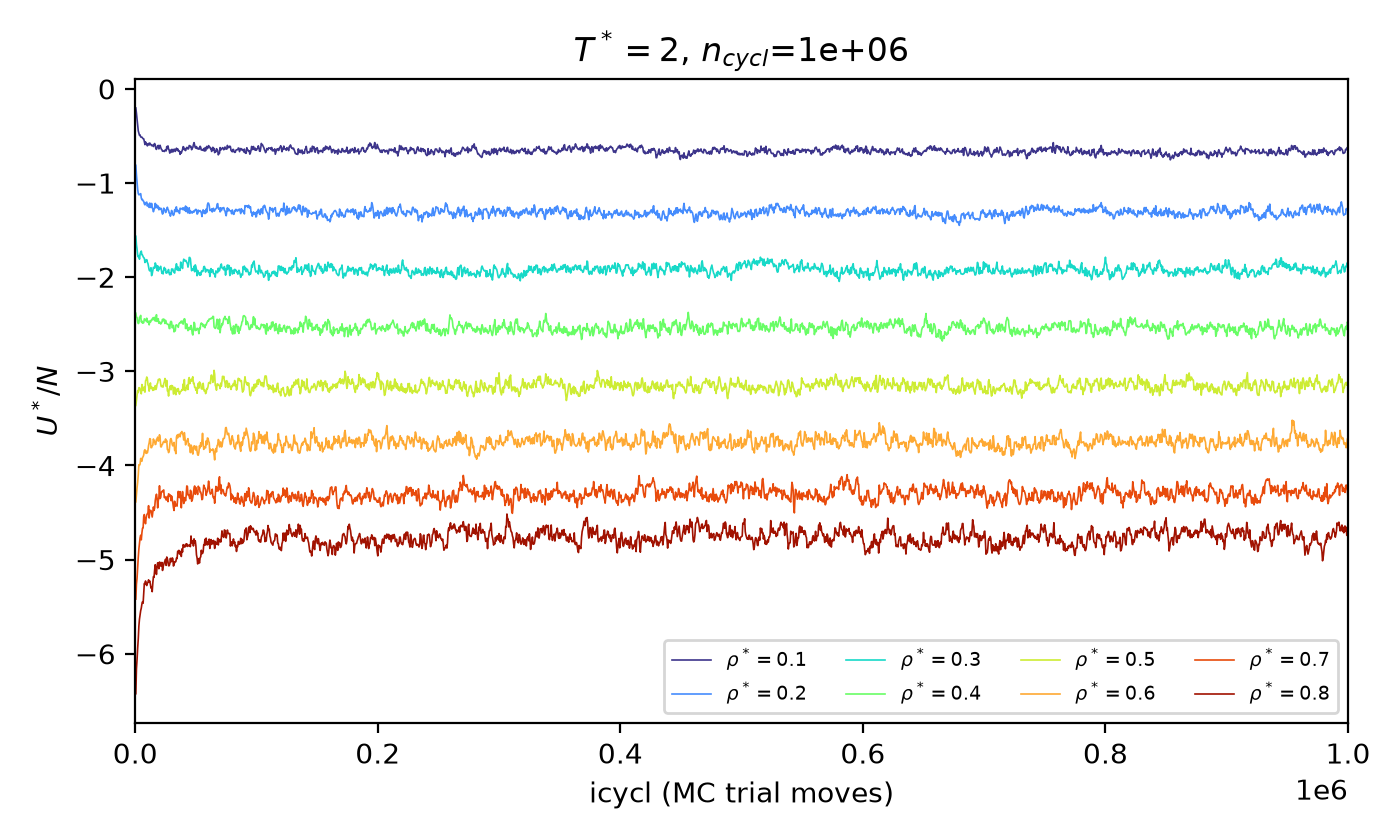
\includegraphics[width=0.8\linewidth]{../figures/U_vs_icycl.png}
  \caption{Sampled $U^*/N$ as a function of the MC move counter \texttt{icycl} for all densities ($T^*=2.0$, $n_{\mathrm{cycl}}=10^6$, fcc start).}
  \label{fig:uicycl}
\end{figure}

\begin{figure}[H]
  \centering
  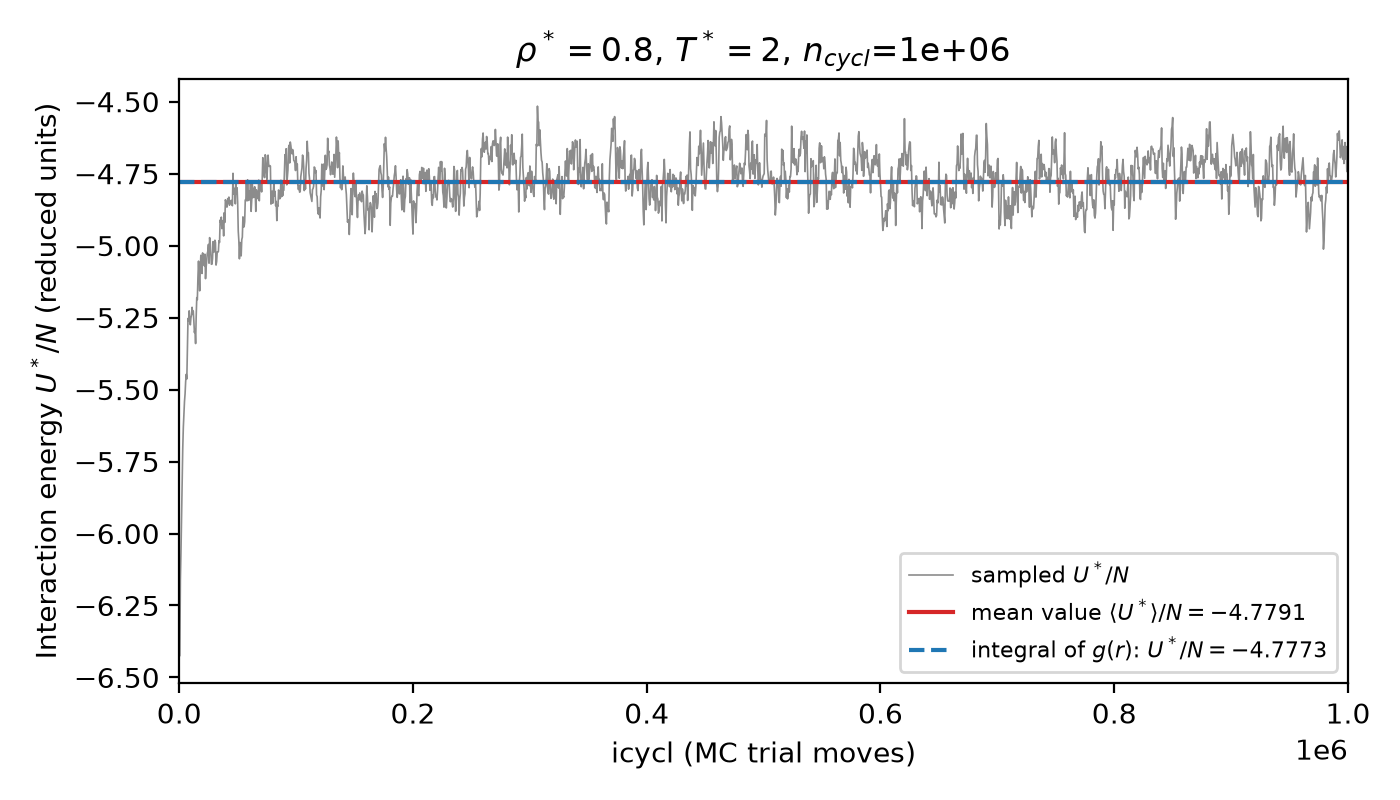
\includegraphics[width=0.8\linewidth]{../figures/U_icycl_rho08.png}
  \caption{Interaction energy $U^*/N$ along the run at $\rho^*=0.8$ ($T^*=2.0$, $n_{\mathrm{cycl}}=10^6$), with the mean value of the samples (solid) and the value from the integral of $g(r)$ (dashed, Step~7).}
  \label{fig:u08}
\end{figure}

\begin{figure}[H]
  \centering
  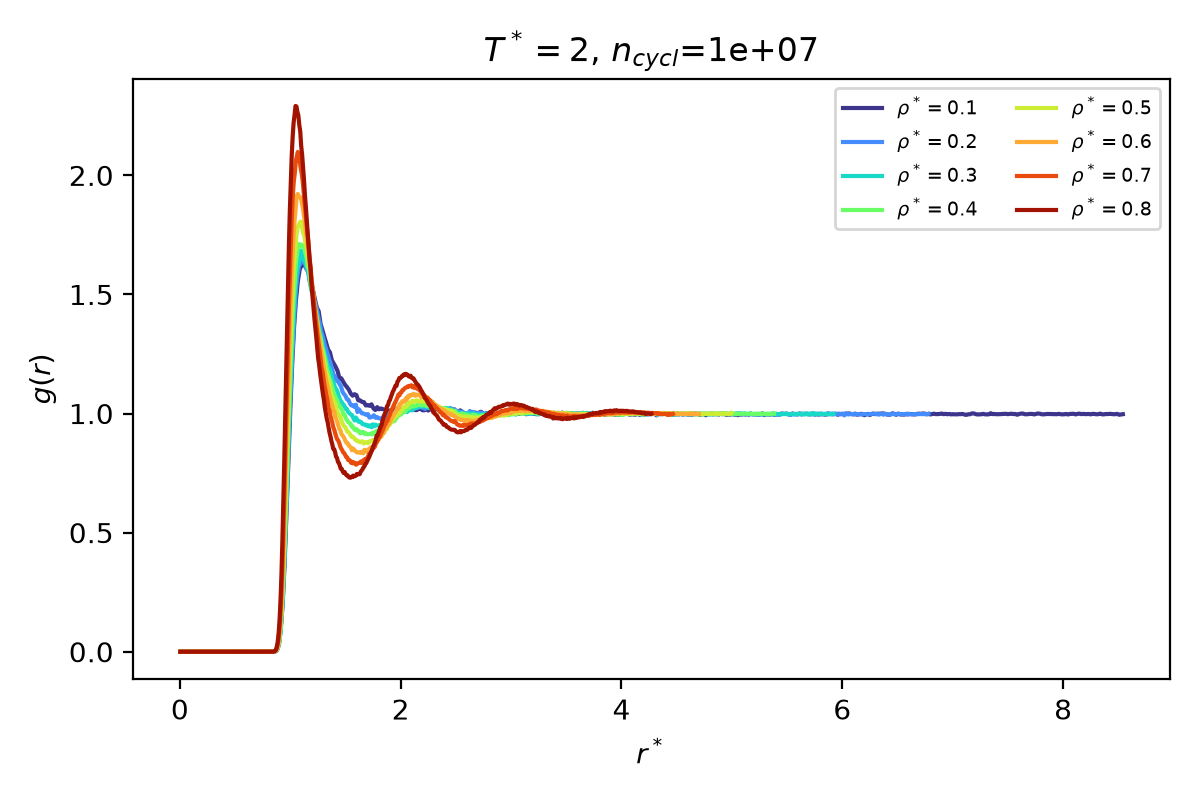
\includegraphics[width=0.7\linewidth]{../figures/gdr.png}
  \caption{Radial distribution function $g(r)$ for $\rho^*=0.1$--$0.8$ ($T^*=2.0$, $10^7$ cycles).}
  \label{fig:gdr}
\end{figure}

\clearpage
\subsection{Discussion \& Notes}
% RESPONSABLE: Torret
For $\rho^*\ge0.4$ we chose $\Delta^*$ so that $43$ to $48\%$ of the moves are accepted. At low density the atoms rarely meet and most moves are accepted ($77\%$ at $\rho^*=0.1$), so the value of $\Delta$ matters little there. Our cutoff of $2.5\sigma$ is shorter than the $4$ to $5\sigma$ of Johnson \emph{et al.}, and the tail corrections make up for it. $\sigma_U$ and $\sigma_P$ grow with $\rho^*$ and barely change with $n_{\mathrm{cycl}}$ ($0.049$ and $0.051$ for $U$ at $\rho^*=0.5$). The $10^6$ and $10^7$ averages of $P$ differ by at most $0.7\%$ up to $\rho^*=0.7$ and by $1.9\%$ at $\rho^*=0.8$. Figure~\ref{fig:uicycl} explains the larger gap at $\rho^*=0.8$: from the fcc start, $U^*/N$ reaches its plateau in about $2\times10^4$ moves for $\rho^*\le0.6$, but needs about $5\times10^4$ at $\rho^*=0.8$, which is $5\%$ of a $10^6$ run and stays in its average.

% RESPONSABLE: Montull
Step~5. In Figure~\ref{fig:eos}, $U^*/N$ goes down from $-0.66$ to $-4.76$ as each atom gets more neighbours inside the attractive well. $P^*$ grows slowly up to $\rho^*\approx0.5$ and then much faster, from $1.07$ to $5.25$, once the repulsive cores start to touch. Both curves have the shape of the figure in Frenkel and Smit. Table~\ref{tab:ideal} shows that the ideal-gas law fails over most of the range. At $\rho^*=0.1$ the pressure is already $11\%$ below $\rho^*T^*$, because the attraction lowers it, and the gap reaches $-18\%$ at $\rho^*=0.2$ and $0.3$. Near $\rho^*=0.45$ the curve crosses the ideal line, where attraction and repulsion cancel, so $Z$ is close to $1$ at $\rho^*=0.5$ ($+7\%$) only by coincidence; $Z$ then rises to $3.3$ at $\rho^*=0.8$. The ideal gas is within $10\%$ only up to $\rho^*\approx0.1$; above that the second virial coefficient is needed.

% RESPONSABLE: Montull
Table~\ref{tab:johnson} compares our results with Johnson \emph{et al.}: $P^*$ agrees within about $1\%$ at every density and $U^*/N$ within $0.3\%$ ($-3.152$ against $-3.149$ at $\rho^*=0.5$). The remaining differences come from our shorter cutoff (the tail correction takes $g=1$ beyond $2.5\sigma$, which is not exact at high density), from the finite size $N=500$ and from the statistics. Johnson \emph{et al.}\ give no value at $\rho^*=0.3$.

% RESPONSABLE: Torret
Step~6. Figure~\ref{fig:gdr} goes from a gas to a dense fluid. At $\rho^*=0.1$, $g(r)$ has a single weak peak of height $1.63$ at $r=1.12$, close to the minimum of the potential at $2^{1/6}$. With increasing density the first peak grows ($1.68$, $1.81$ and $2.29$ at $\rho^*=0.3$, $0.5$ and $0.8$) and moves inwards from $1.12$ to $1.05$ as the fluid is compressed, and more shells appear at the highest densities. At every density $g$ tends to $1$ at large $r$ (between $0.997$ and $1.000$ in the last bins), as the tail correction assumes. Because $T^*=2$ is high, the structure is softer than that of the liquid at $T^*=0.71$ in Practice~2, whose first peak reached $3.0$.

% RESPONSABLE: Montull
Step~7. Table~\ref{tab:integral} shows that integrating $g(r)$ gives the same values as the direct averages: $|\Delta U|\le0.002$, below $0.1\%$ of $U$, and $|\Delta P|\le0.008$, at most $0.3\%$ and always above the direct value. Both routes use the same configurations, so the difference is numerical and comes from the bin width ($L/1000$) in the rectangle rule. $P$ is more sensitive because $r^3\,dU/dr$ is largest in the steep repulsive region. Figure~\ref{fig:u08} shows this for the densest run: the two horizontal lines ($-4.7791$ and $-4.7773$) are closer than the width of the line, while the samples fluctuate around them with $\sigma_U=0.13$.

% RESPONSABLE: Montull
\textbf{Conclusion.} Our MC code reproduces the Lennard-Jones equation of state at $T^*=2.0$ within about $1\%$ of Johnson \emph{et al.} The ideal-gas law holds only up to $\rho^*\approx0.1$, and integrating $g(r)$ gives the same $U$ and $P$ as the direct averages within $0.3\%$.

% RESPONSABLE: Torret (Annex: codigo completo)
\clearpage
\thispagestyle{empty}
\null
\vspace*{\fill}
\begin{center}
{\fontsize{48}{58}\selectfont\bfseries Annex}
\end{center}
\vspace*{\fill}
\clearpage
Full source of the Monte Carlo program.

\lstinputlisting[style=fortranstyle,caption={Full program \texttt{mcnvt.f90}.},label={lst:full}]{../antislop/mcnvt.f90}
\end{document}
